\documentclass{article}
\usepackage{xepersian}
\usepackage{listings}
\usepackage{xcolor}
\usepackage{graphicx}
\usepackage{caption}
\usepackage[margin=3.6cm]{geometry}

\lstset{
    tabsize = 4,
    showstringspaces = false,
    commentstyle = \color{green},
    keywordstyle = \color{blue},
    stringstyle = \color{red},
    rulecolor = \color{black},
    basicstyle = \small \ttfamily,
    breaklines = true,
}

\settextfont{XB Yas}

\title{\textbf{گزارش‌کار پروژۀ عید - برنامه‌سازی پیشرفته (جاوا)}\vspace{1cm}\\پاسخ سوالات قدم سوم}
\author{\textbf{پیشوا آزیز - \lr{40313003}}}
\date{}

\begin{document}

\maketitle

\vspace{2cm}

\section*{پاسخ سوال ۱}
کلیدواژهٔ \lr{\lstinline{instanceof}} در \lr{Java} برای بررسی این‌که متغیر \lr{reference type} مورد نظر، شامل رفرنس خاصی از آبجکتی دیگر می‌باشد، مورد استفاده قرار می‌گیرد.
این کلیدواژه، یک عمل‌گر مقایسه‌ای به حساب می‌آید به‌طوری که یک \lr{\lstinline{instance}} را با یک \lr{type} مقایسه می‌کند و مقداری از نوع \lr{\lstinline{boolean}} را بازمی‌گرداند. برای مثال، خروجی کد زیر عبارت \lr{\lstinline{true}} است.

\begin{latin}
\begin{lstlisting}[language=Java]
public class Main {
    public static void main(String[] args) {
        Car benz = new Car("Mercedes-Benz");
        boolean check = benz instanceof Car;
        System.out.println(check);
    }
}

class Car {
    String brand;
    public Car(String brand) {
        this.brand = brand;
    }
}

\end{lstlisting}
\end{latin}

در اینجا آبجکتی از نوع \lr{\lstinline{Car}} ایجاد شده است و با استفاده از کلیدواژهٔ \lr{instanceof}، بررسی شده است که آیا از نوع \lr{\lstinline{Car}} می‌باشد یا نه، که طبیعتاً درست خواهد بود و مقدار \lr{\lstinline{true}} در متغیر \lr{\lstinline{check}} ذخیره می‌شود.

\section*{پاسخ سوال ۲}
یکی دیگر از روش‌های \lr{validate} کردن مقادیر فیلدهای اعضای دیتابیس استفاده از شرط‌های مربوطه در داخل متدهای \lr{\lstinline{add}} و \lr{\lstinline{update}} می‌باشد که در مقابل روش استفاده از \lr{\lstinline{Validator}}ها، معایب بسیار زیادی دارد. یکی از معایب این روش این است که اصول \lr{clean code} همچون خوانایی کد، نگه‌داری و \lr{dynamic} بودن یا پویایی آن، رعایت نمی‌شود. به‌طوری که در آینده برای گسترش کد و اضافه کردن فیلدها و ویژگی‌های بیشتر به \lr{\lstinline{Entity}}ها، باید شرط‌های جدید برای \lr{validate} کردن آن‌ها اضافه شود.

\section*{پاسخ سوال ۳}

\begin{figure}[h]
    \centering
    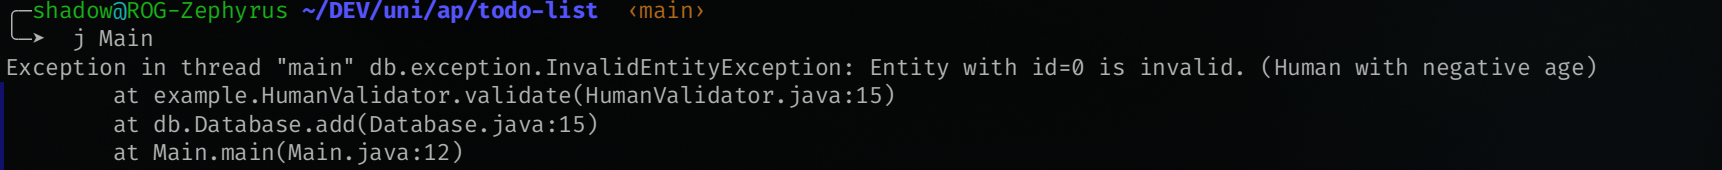
\includegraphics[width=1\textwidth]{../img/screenshot2.png}
    \caption*{اسکرین‌شات از خروجی کد حین اجرای بخش تست کد}
\end{figure}

\end{document}
